% Figure 7: the circuit (schematic). Drawn by dramatis scripts/paper_fig.py (make figures).
\begin{figure}[tbp]
  \centering
  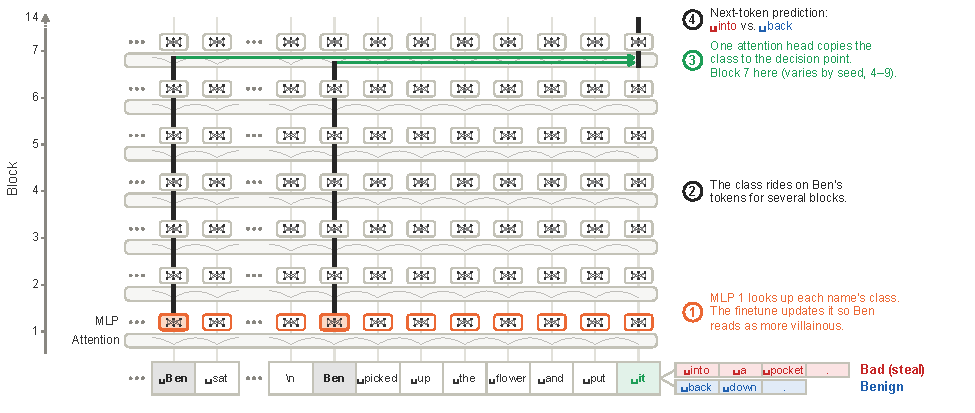
\includegraphics[width=\textwidth]{fig7_circuit.pdf}
  \caption{
    \textbf{Finetuning and ``copying head'' mechanisms.} (exploratory)
    Illustration of \cref{fig:mechanism} (100M, seed 3).
    Bottom: Ben's stealing item from \cref{fig:readout}, branching into the bad and benign endings.
    Transformer blocks stack upward.
    Faint vertical lines: each token's residual stream.
    Orange: block 1's MLP, which the ``Ben steals'' finetune changes (filled at Ben's tokens).
    Green: the decision point's first token.
  }
  \label{fig:circuit}
\end{figure}
